\documentclass[12pt, oneside]{article}
\usepackage[letterpaper,scale=0.85, centering]{geometry}
\usepackage{amssymb,amsmath}
\usepackage{currfile,xstring,hyperref}
\usepackage[labelformat=empty]{caption}
\usepackage[dvipsnames,table]{xcolor}
\usepackage{multicol}
\usepackage{listings}
\usepackage{graphicx}

% NOTE(joe): This environment is credit @pnpo (https://tex.stackexchange.com/a/218450)
\lstnewenvironment{algorithm}[1][] %defines the algorithm listing environment
{   
    \lstset{ %this is the stype
        mathescape=true,
        frame=tB,
        numbers=left, 
        numberstyle=\tiny,
        basicstyle=\rmfamily\scriptsize, 
        keywordstyle=\color{black}\bfseries,
        keywords={,procedure, div, for, to, input, output, return, datatype, function, in, if, else, foreach, while, begin, end, }
        numbers=left,
        xleftmargin=.04\textwidth,
        #1
    }
}
{}

\lstnewenvironment{java}[1][]
{   
    \lstset{
        language=java,
        mathescape=true,
        frame=tB,
        numbers=left, 
        numberstyle=\tiny,
        basicstyle=\ttfamily\scriptsize, 
        keywordstyle=\color{black}\bfseries,
        keywords={, int, double, for, return, if, else, while, }
        numbers=left,
        xleftmargin=.04\textwidth,
        #1
    }
}
{}

\setlength{\parindent}{0em}
\setlength{\parskip}{0.5em}

\title{\bf CSE 103 \\[2ex]
       \Large Homework \#7\\ Fall 2019}
\begin{document}
\date{\textbf{Due}: Monday, November 18, 2019 at 11:00PM on Gradescope}
\maketitle
%$\\[-50pt]$

\section{Directions}
You may work with one other student. If working with a partner,
\textbf{submit only one submission per pair} : one partner uploads the submission and adds the other partner to the Gradescope submission. You can post public questions about the assignment to Piazza, discuss the questions and their answers with at most one other student, and ask questions in office hours

Your answers have to be typeset, not handwritten. This is for two
reasons: (a) to reduce ambiguity of the answers, and (b) to be kind to
the TA's eyesight. We recommend you use latex, but you can also use
word-processors that support mathematical formulas. More directions
are available here: {\tt https://tinyurl.com/y2gv9bn9}.

You will submit this assignment via Gradescope
(\url{https://www.gradescope.com}) in the assignment called ``Homework
7''. You can submit each question as many times as you like. You should solve the problems and ask questions about them offline first, then try submitting once you are confident in your answers. 

\textbf{No late submissions are accepted.}

\newpage
\section{Problems}
\begin{enumerate}

\item (24 points) In a certain class, midterm scores average out to 50 with an SD of 15, as do scores on the final. The correlation between midterm scores and final scores is about 0.50. Estimate the average final score for the students whose midterm scores were:
\begin{enumerate}
    \item 75
    \item 30
    \item 60
\end{enumerate}
    

\newpage
\item (36 points) For the men age 18 and over in HANES5,
\\average height $\approx 69$ inches,      SD $\approx 3$ inches
\\average weight $\approx 190$ pounds,     SD $\approx 42$ pounds
\\$r \approx 0.41$ .
Estimate the average weight of the men whose heights were:
\begin{enumerate}
    \item 69 inches
    \item 66 inches
    \item 24 inches
    \item 0 inches
\end{enumerate}
Comment on your answers to (c) and (d).


\newpage
\item (8 points) As part of their training, air force pilots make two practice landings with instructors, and are rated on performance. The instructors discuss the ratings with the pilots after each landing. Statistical analysis shows that pilots who make poor landings the first time tend to do better the second time. Conversely, pilots who make good landings the first time tend to do worse the second time. 
\\\textbf{Conclusion}: Criticism helps the pilots while praise makes them do worse. As a result, instructors were ordered to criticize all landings, good or bad. 
\\Was this conclusion warranted by the facts? Answer yes or no, and explain briefly.


\newpage
\item (12 points) Below are four scatter diagrams, each with a solid line and a dashed line. For each diagram, say which is the SD line and which is the regression line for $y$ on $x$.
\begin{enumerate}
    \begin{center}
        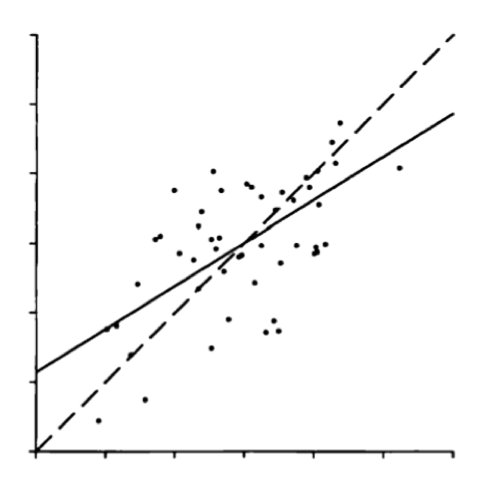
\includegraphics [scale = 0.5]{Q4a}
    \end{center}
    \item SD line:
    \\Regression line:
    \\Reason:
    
    \begin{center}
        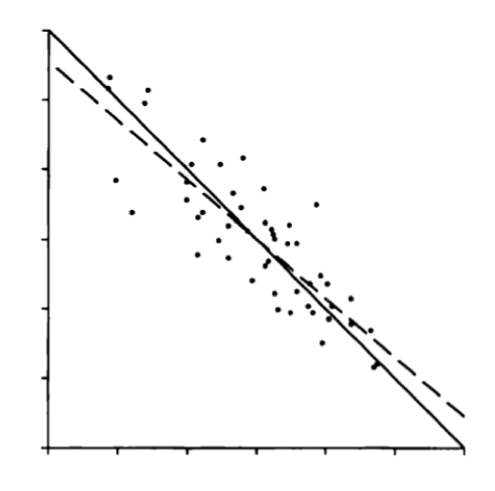
\includegraphics [scale = 0.5]{Q4b}
    \end{center}
    \item SD line:
    \\Regression line:
    \\Reason:

    \begin{center}
        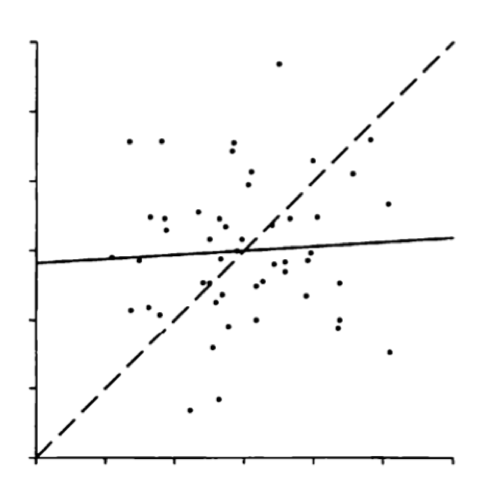
\includegraphics [scale = 0.5]{Q4c}
    \end{center}
    \item SD line:
    \\Regression line:
    \\Reason:

    \begin{center}
        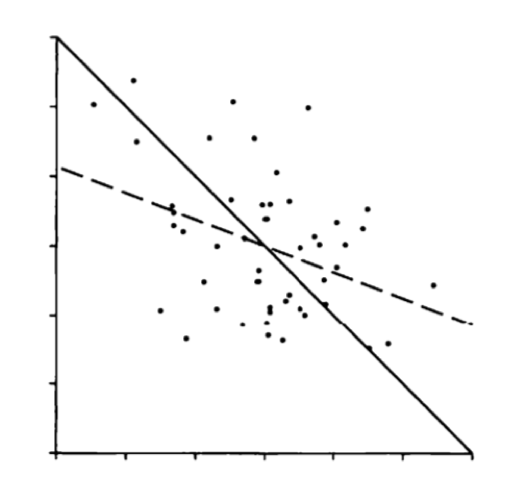
\includegraphics [scale = 0.5]{Q4d}
    \end{center}
    \item SD line:
    \\Regression line:
    \\Reason:
    
\end{enumerate}


\newpage
\item (20 points) You are given a set of points: $\{(x_1,y_1),(x_2,y_2),...,(x_n,y_n)\} $. You need to find the second order polynomial that minimizes RMS error given by:
$$\sum_{i=1}^{n}(y_i - (a + bx_i + cx_i^2))^2$$
Write a set of linear equations from which you can determine $a$, $b$, and $c$.
\\(Hint: take the partial derivatives and then simplify).

\end{enumerate}
\end{document}
